\documentclass[runningheads]{llncs}
%
\usepackage{graphicx}
\usepackage[spanish,es-tabla]{babel}
\usepackage[utf8]{inputenc}
\usepackage{float} % para la posición en la pagina
\usepackage{multirow} % para las tablas
\setlength{\tabcolsep}{0.5em} % padding horizontal tablas
\graphicspath{ {./graficos/} } % ruta de las graficas
\usepackage{enumerate} % centrar listas

% Used for displaying a sample figure. If possible, figure files should
% be included in EPS format.

\begin{document}
%
\title{Análisis de algoritmos de búsqueda aplicados al problema del 8-puzzle}

\author{José Antonio García García. \email{UO251317@uniovi.es}}

\institute{Sistemas Inteligentes. Grado en Ingeniería Informática. EII. Universidad de Oviedo. Campus de los Catalanes. E-33007. Oviedo}
%
\maketitle              % typeset the header of the contribution
%
\begin{abstract}
Se estudia la resolución del problema del 8-puzzle mediante algoritmos de búsqueda en espacios de estados, y la resolución del Travelling Salesman Problem (TSP) mediante búsqueda heurística y Algoritmos Genéticos (AGs). Para ello, se considerarán algunos de los algoritmos más conocidos, tanto no informados (búsqueda en anchura, profundidad, etc.) como informados (A*, PEA*, ...) considerando distintos heurísticos, o el AG simple. En los experimentos se utilizan las implementaciones de estos algoritmos incluidas en el software aima-java. Mediante un estudio experimental se analizan las propiedades de estos algoritmos, contrastando los resultados con la teoría.

\keywords{8-puzzle \and heurísticos \and búsqueda en espacios de estados \and búsqueda a ciegas \and recorrido en anchura \and recorrido en profundidad \and recorrido con coste uniforme \and búsqueda recursiva \and recorrido en profundidad \and A* \and búsqueda inteligente \and búsqueda en árboles \and búsqueda en grafos \and búsqueda en grafos con re-expansión \and búsqueda en grafos con rectificación \and ponderación estática de A* \and recorrido Greedy Best First \and algoritmos genéticos.}
\end{abstract}
%
%
%
\section{Introducción}

El software aima-java, que implementa los algoritmos descritos en~\cite{referencia_Russell}, viene preparado para su uso desde varios entornos, entre ellos Eclipse. Para utilizarlo, se descomprime el fichero aima-java.zip en un directorio (el original se puede descargar de la página oficial http://code.google.com/p/aima-java/).

Luego se arranca el entorno Eclipse y se elige dicho directorio como workspace. Se importan dos proyectos “General/Existing Projects into Workspace” con los directorios aima-core y aima-gui. A continuación, se lanza la ejecución como “java application” y, si lo que queremos es experimentar con prototipos de búsqueda en espacios de estados, se selecciona entre varias demos la que se llama EigthPuzzleDemo. Esta demo lanza la ejecución de varios algoritmos de búsqueda sobre la misma instancia del problema, considerando búsqueda en árboles o búsqueda en grafos.

A partir de ahí se trata de ir ejecutando de uno en uno los algoritmos de búsqueda sobre distintas instancias del problema. Para ver cómo se hace esto hay que editar el código de la demo anterior, que está en el fichero EigthPuzzleDemo.java, y seleccionar el algoritmo de búsqueda, comentando las llamadas al resto de algoritmos, así como el estado inicial.

En las siguientes secciones se describirán con más detalle los apartados en los que se ha dividido este estudio: en la sección~\ref{seccion_ciega} los algoritmos de búsqueda ciega, en la sección~\ref{seccion_inteligente} los algoritmos de búsqueda inteligente, en la sección~\ref{seccion_problema} el problema del 8-puzzle, en la sección~\ref{seccion_estudio} los datos del estudio y en la sección~\ref{seccion_conclusion} la deducción obtenida a partir del estudio.


\section{Algoritmos de Búsqueda a Ciegas}\label{seccion_ciega}

Los algoritmos de búsqueda a ciegas no utilizan conocimiento o información específica del dominio del problema ~\cite{referencia_Busqueda_Ciegas}, es decir, son aquellos que realizan un recorrido del espacio de búsqueda de una forma metódica sin analizar el dominio del problema que se les plantea.

En este articulo veremos las tres 3 opciones que hay disponibles para este tipo de casos:
\begin{enumerate}[\hspace{2cm}]
\item · Búsqueda en profundidad.
\item · Búsqueda en anchura.
\item · Búsqueda con coste uniforme. 
\end{enumerate}

\section{Algoritmos de Búsqueda Inteligente}\label{seccion_inteligente}

En contraposición al anterior sistema de búsqueda se encuentran los algoritmos de búsqueda inteligente, que utilizan, dentro del funcionamiento del algoritmo de búsqueda, conocimiento adicional sobre el problema que se está intentando resolver. A esta información se le conoce como heurístico y es el encargado de asignar un coste al camino desde un nodo hasta el nodo objetivo.

\subsection{El algoritmo A*}

El algoritmo A* fue propuesto por Peter E. Hart, Nils J. Nilsson y Bertram Raphael en ~\cite{referencia_Korf_9} y está muy bien descrito en ~\cite{referencia_Nilsson} y sobre todo en ~\cite{referencia_Pearl}. El objetivo de este algoritmo es lograr encontrar la solución óptima expandiendo el menor número de nodos posibles.

El algoritmo A* esta definido por la función de evaluación f(n), siendo ésta una aproximación de f*(n), que se define como la función del coste mínimo del nodo inicial a los objetivos condicionado a pasar por n. Para calcular f(n) es necesario conocer el mejor coste desde el nodo inicial hasta un nodo n, a lo que se llama g(n) y el heurístico a utilizar, al cual nos referiremos como h(n). De esta forma el algoritmo A* se definiría como:

\begin{equation}
f(n) = g(n) + h(n)
\end{equation}

\subsection{Ponderación estática PEA*}

Como variante del algoritmo A* se desarrolló el algoritmo de ponderación estática (PEA*). Este nuevo algoritmo tiene un error acotado, no es admisible y es de la forma:

\begin{equation}
f(n) = g(n) + (1 + \varepsilon) * h(n)
\end{equation}

En esta formula $\varepsilon$ es el error acotado que se indica para calcular el nuevo coste.

\subsection{Greedy Best-First Search}

Este caso en concreto se trata de un algoritmo voraz cuya función de estimación es:

\begin{equation}
f(n) = h(n)
\end{equation}

Para más información revisar las referencias ~\cite{referencia_Russell} y ~\cite{referencia_Geek}

\section{El problema del 8-puzzle}\label{seccion_problema}

El problema del 8-puzzle es uno de los ejemplos de referencia a la hora de probar y/o explicar los algoritmos de búsqueda, es por está razón que lo usaremos en nuestros experimentos.

\subsection{Enunciado del problema}

Para el problema del 8-puzzle se usa un cuadrado con 8 celdas cuadradas en su interior distribuidas en forma de un tablero de 3x3 dimensiones. El cuadrado restante está sin rellenar. Cada bloque tiene un número del 1 al 8.

El problema consiste en ordenar los números para alcanzar un estado objetivo. Las celdas unicamente se pueden mover de forma ortogonal a una celda vacía si esta se encuentra adyacente.

\subsection{Modelado en el marco de búsqueda en espacios de estados}

Se parte de un estado inicial desde el que se empezará a resolver el problema y se tratará del alcanzar un estado objetivo, el cual se debé indicar al inicio de la resolución. 

Para enmarcar el problema trataremos cada estado del grafo como un nodo y, teniendo en cuenta que los movimientos son reversibles, enmarcaremos el problema dentro de un grafo. Por esta razón cada estado del problema se encuentra definido por la disposición de las celdas en ese momento.

\subsection{Heurísticos}

La siguiente lista contiene los heurísticos utilizados en los experimentos:
\begin{enumerate}[\hspace{1cm}]
\item · $h_0$: Su heurístico es nulo. En el documento se le hace referencia como "Nulo".
\item · $h_1$: Se basa en contar el número de fichas fuera de lugar. En el documento se le hace referencia como $"$Casilla fuera de lugar".
\item · $h_{1-2}$: Se basa en sumar 0 si la fila está en su lugar, 1 si la ficha no esta en la columna o fila correcta y 2 si no se cumple ninguno de los dos escenarios. En el documento se le hace referencia como $"$Coincidencia Fila Columna".
\item · $h_2$: Se basa en la suma de las distancias ortogonales de cada celda a la posición que le corresponde. En el documento se le hace referencia como "Manhattan".
\item · $h_3$: Se basa en la distancia ortogonal a distancia 2 de cada celda a su posición final. En el documento se le hace referencia como $"$Inconsistente".
\item · $h_4$: Se basa en la formula de Stern en este artículo ~\cite{referencia_Stern}.  En el documento se le hace referencia como $"$RoniStern". Su formula es la siguiente:

\begin{equation}
f(n) = max ( h_2(n) , 1.31 * h_2(n) - 2.19)
\end{equation}

\end{enumerate}

\section{Estudio experimental}\label{seccion_estudio}

Para la realización de nuestro estudio hemos tenido en cuenta varios casos de prueba y se ha hecho la media de todos ellos para así asegurarnos de la veracidad de los datos y que estos se vean afectados en menor medida por procesos que se estén ejecutando en segundo plano en el ordenador sobre el que se realizan las pruebas.

\subsection{Banco de ejemplos}

Para la realización de las pruebas se han utilizado 3 variantes, del mismo coste, diferentes. Cada variante representa de esta forma una caso de prueba y se ve ligado a otros dos casos de prueba en función de su coste. En la \textbf{Tabla \ref{tabla_banco_ejemplos}} se encuentran los casos de prueba utilizados en el estudio.

\begin{table}[H]
\centering
\caption{Casos de prueba con los que se realizaron las pruebas ordenados por costes.}\label{tabla_banco_ejemplos}
{\renewcommand{\arraystretch}{1.8}
\begin{tabular}{|c|c|c|c|}
\hline
\#coste &  \multicolumn{3}{|c|}{Caso}\\
\hline
  & Número 1 & Número 2 & Número 3\\
\hline\hline
5 & \{1, 2, 3, 0, 4, 5, 8, 7, 6\} & \{1, 0, 2, 8, 6, 3, 7, 5, 4\} & \{2, 8, 3, 1, 6, 4, 7, 0, 5\}\\
\hline
10 & \{1, 3, 4, 6, 7, 2, 0, 8, 5\} & \{3, 2, 4, 1, 0, 5, 8, 7, 6\} & \{8, 1, 0, 2, 5, 3, 7, 4, 6\}\\
\hline 
15 & \{6, 3, 5, 2, 1, 0, 8, 4, 7\} & \{6, 0, 3, 8, 1, 5, 4, 2, 7\} & \{7, 8, 3, 1, 5, 0, 4, 2, 6\}\\
\hline 
20 & \{1, 4, 7, 6, 8, 5, 0, 3, 2\} & \{6, 4, 0, 2, 8, 1, 7, 3, 5\} & \{4, 1, 3, 7, 2, 8, 5, 6, 0\}\\
\hline 
25 & \{3, 4, 8, 5, 7, 1, 6, 0, 2\} & \{4, 5, 3, 7, 6, 2, 8, 0, 1\} & \{2, 7, 8, 5, 4, 0, 3, 1, 6\}\\
\hline 
30 & \{5, 4, 7, 6, 0, 3, 8, 2, 1\} & \{3, 8, 7, 4, 0, 6, 5, 2, 1\} & \{5, 6, 3, 4, 0, 2, 7, 8, 1\}\\
\hline
\end{tabular}
}
\end{table}

\subsection{Resultados experimentales}

Para empezar hemos probado y analizado los peores algoritmos sobre el banco de ejemplos; estos son los algoritmos de búsqueda ciega: profundidad, anchura y coste uniforme. Para ello hemos considerado el espacio de búsqueda como un árbol y como un grafo. 

Los datos de la búsqueda en arboles no aparecen en este articulo debido al propio espacio de búsqueda. Al tratarse de una estructura en forma de árbol, es posible entrar en un bucle infinito en las ramas sin obtener ninguna solución por lo que se considero apropiado no mostrarlos.

Por otro lado podemos apreciar que la búsqueda sobre un grafo si ha alcanzado soluciones pero, como se puede ver en la \textbf{Figura \ref{figura_ciega_grafo}} , ni son consistentes ni el número de nodos expandidos es una cantidad viable para problemas grandes.

\begin{figure}
	\centering
	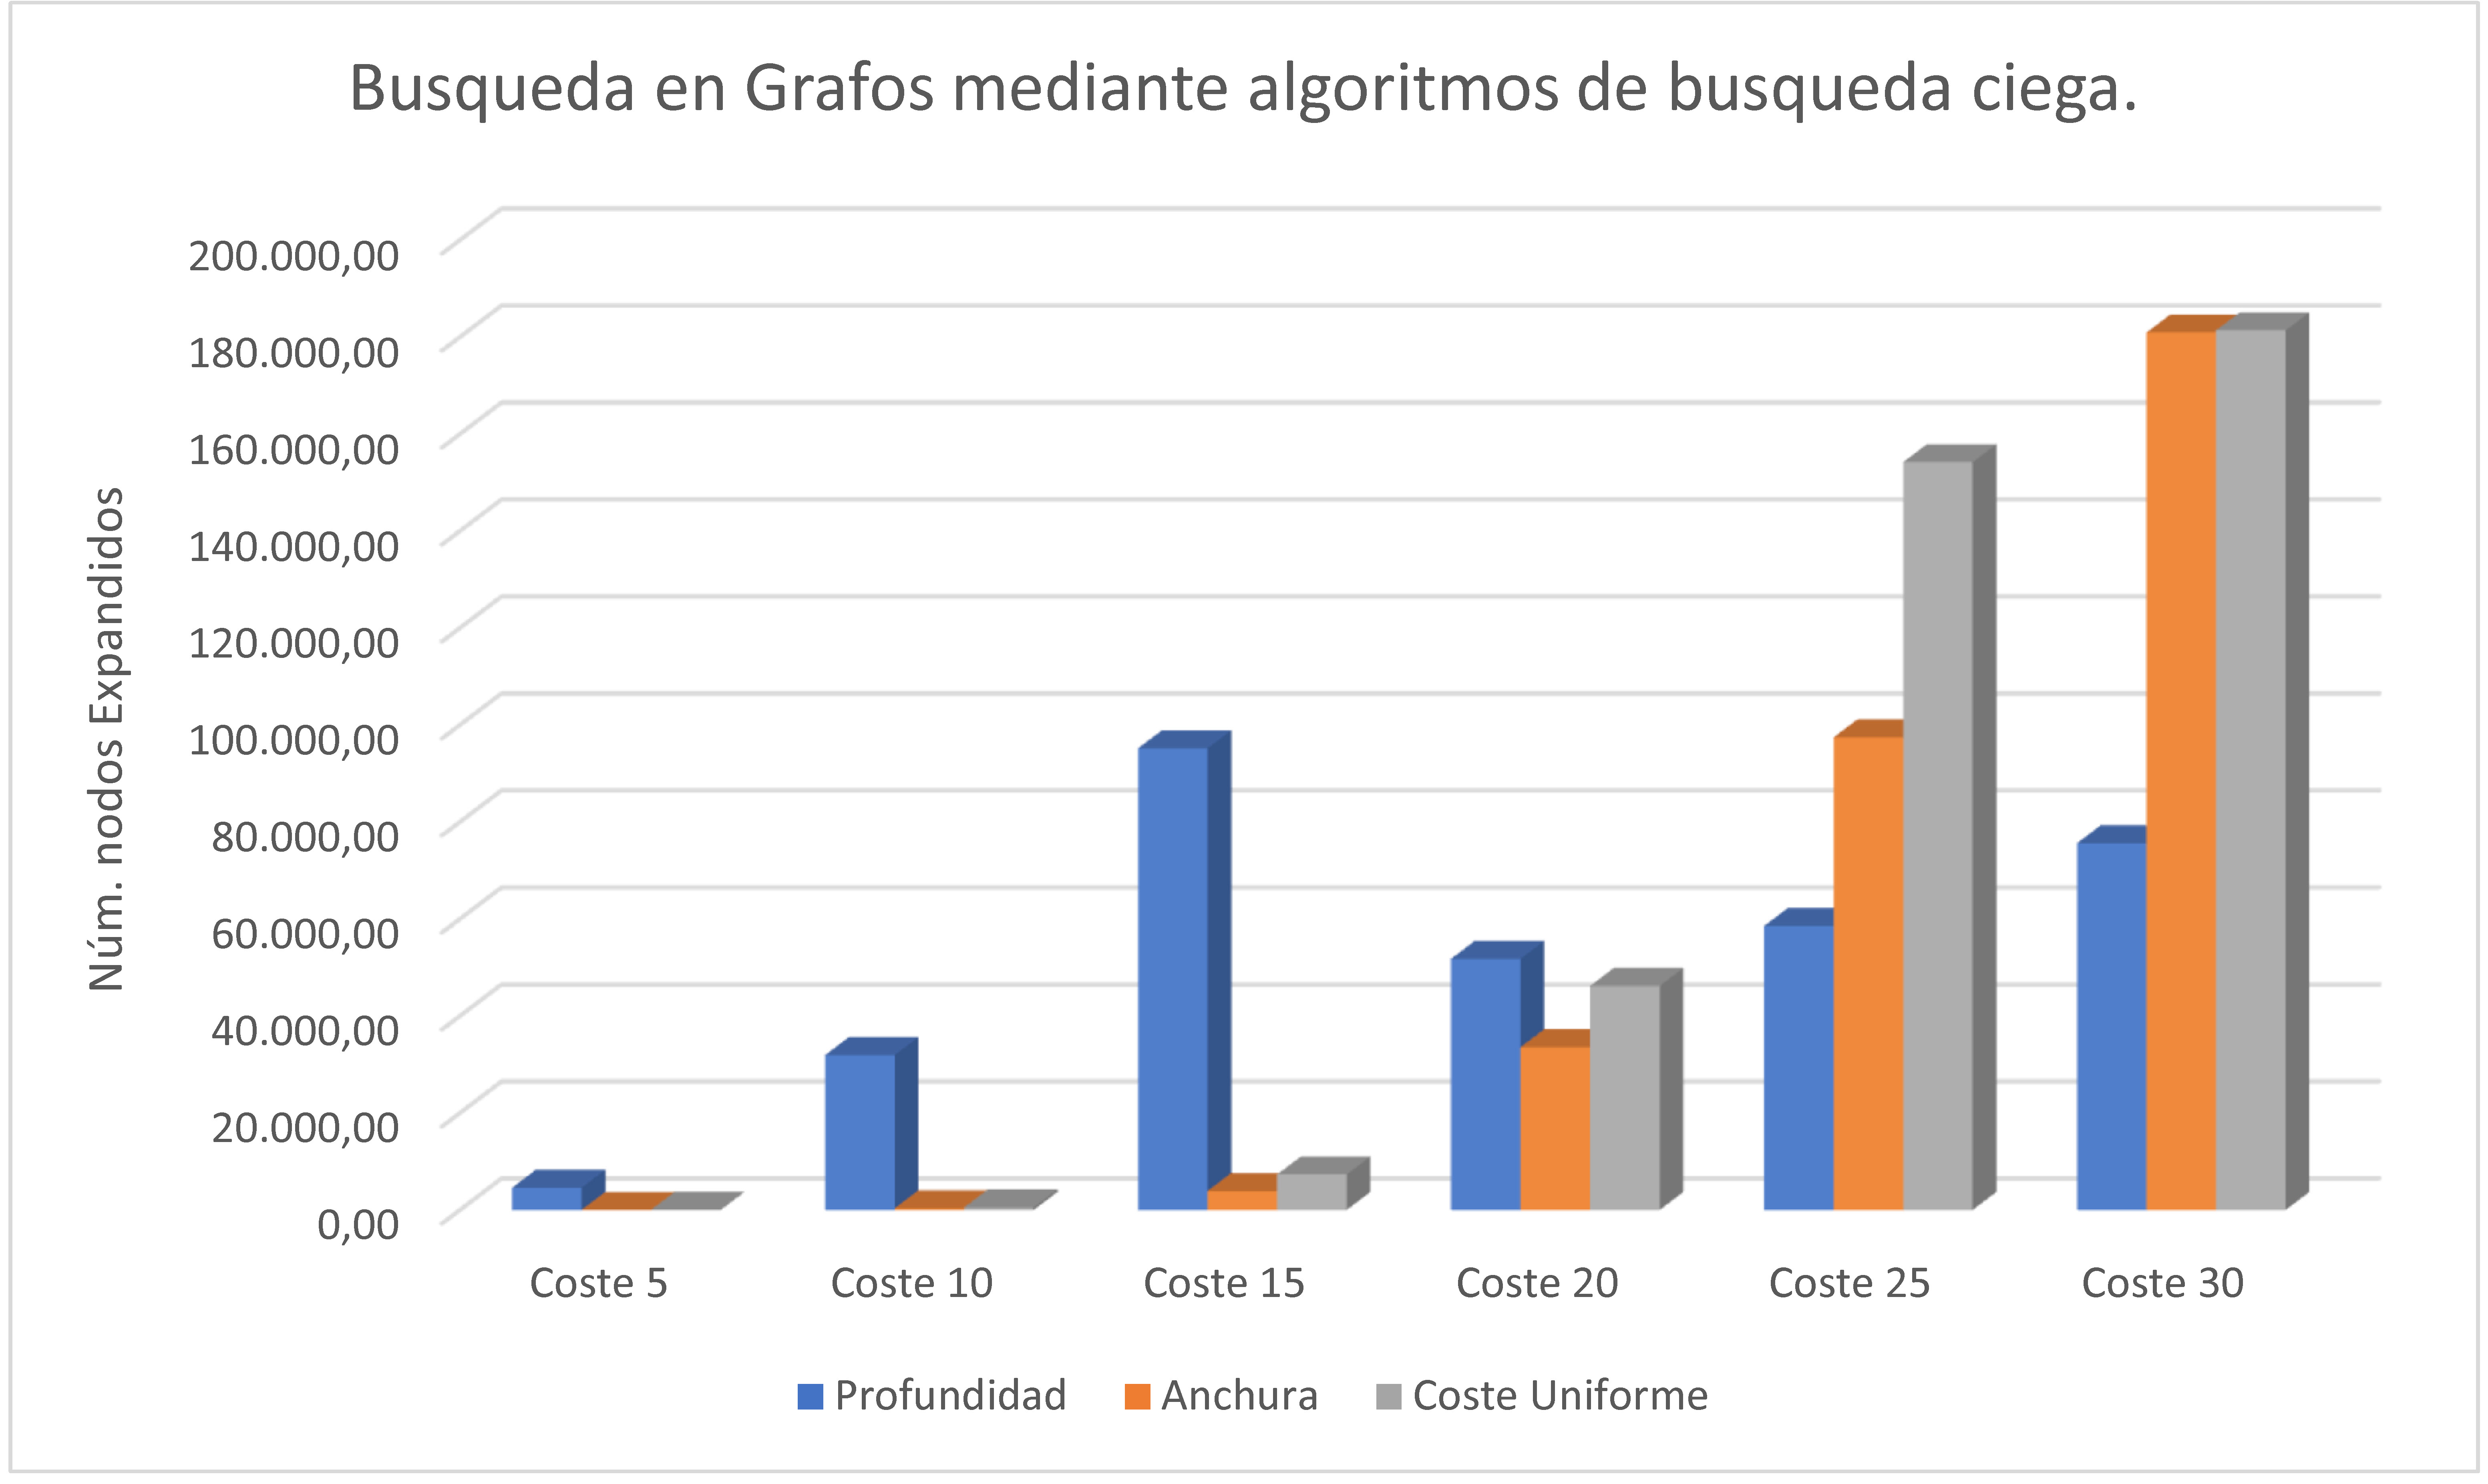
\includegraphics[width=\textwidth]{ejercicio1.jpg}
	\caption{Número medio de nodos expandidos por cada versión de los algoritmos a ciegas sobre búsqueda en grafos.} 
	\label{figura_ciega_grafo}
\end{figure}

Siguiendo los casos anteriores de algoritmos a ciegas, hemos puesto a prueba los algoritmos recursivos de búsqueda en profundidad limitada e iterativa. En la \textbf{Figura \ref{figura_recursiva_grafo}} podemos ver que la versión iterativa no es viable ya que para un problema de coste 15 necesita expandir mas de 3 millones de nodos. Por otro lado la versión limitada, a pesar de no ser tan alta la cantidad de nodos expandidos como la otra versión recursiva, no es capaz de obtener soluciones según aumentan los costes de los ejemplos.

\begin{figure}[H]
	\centering
	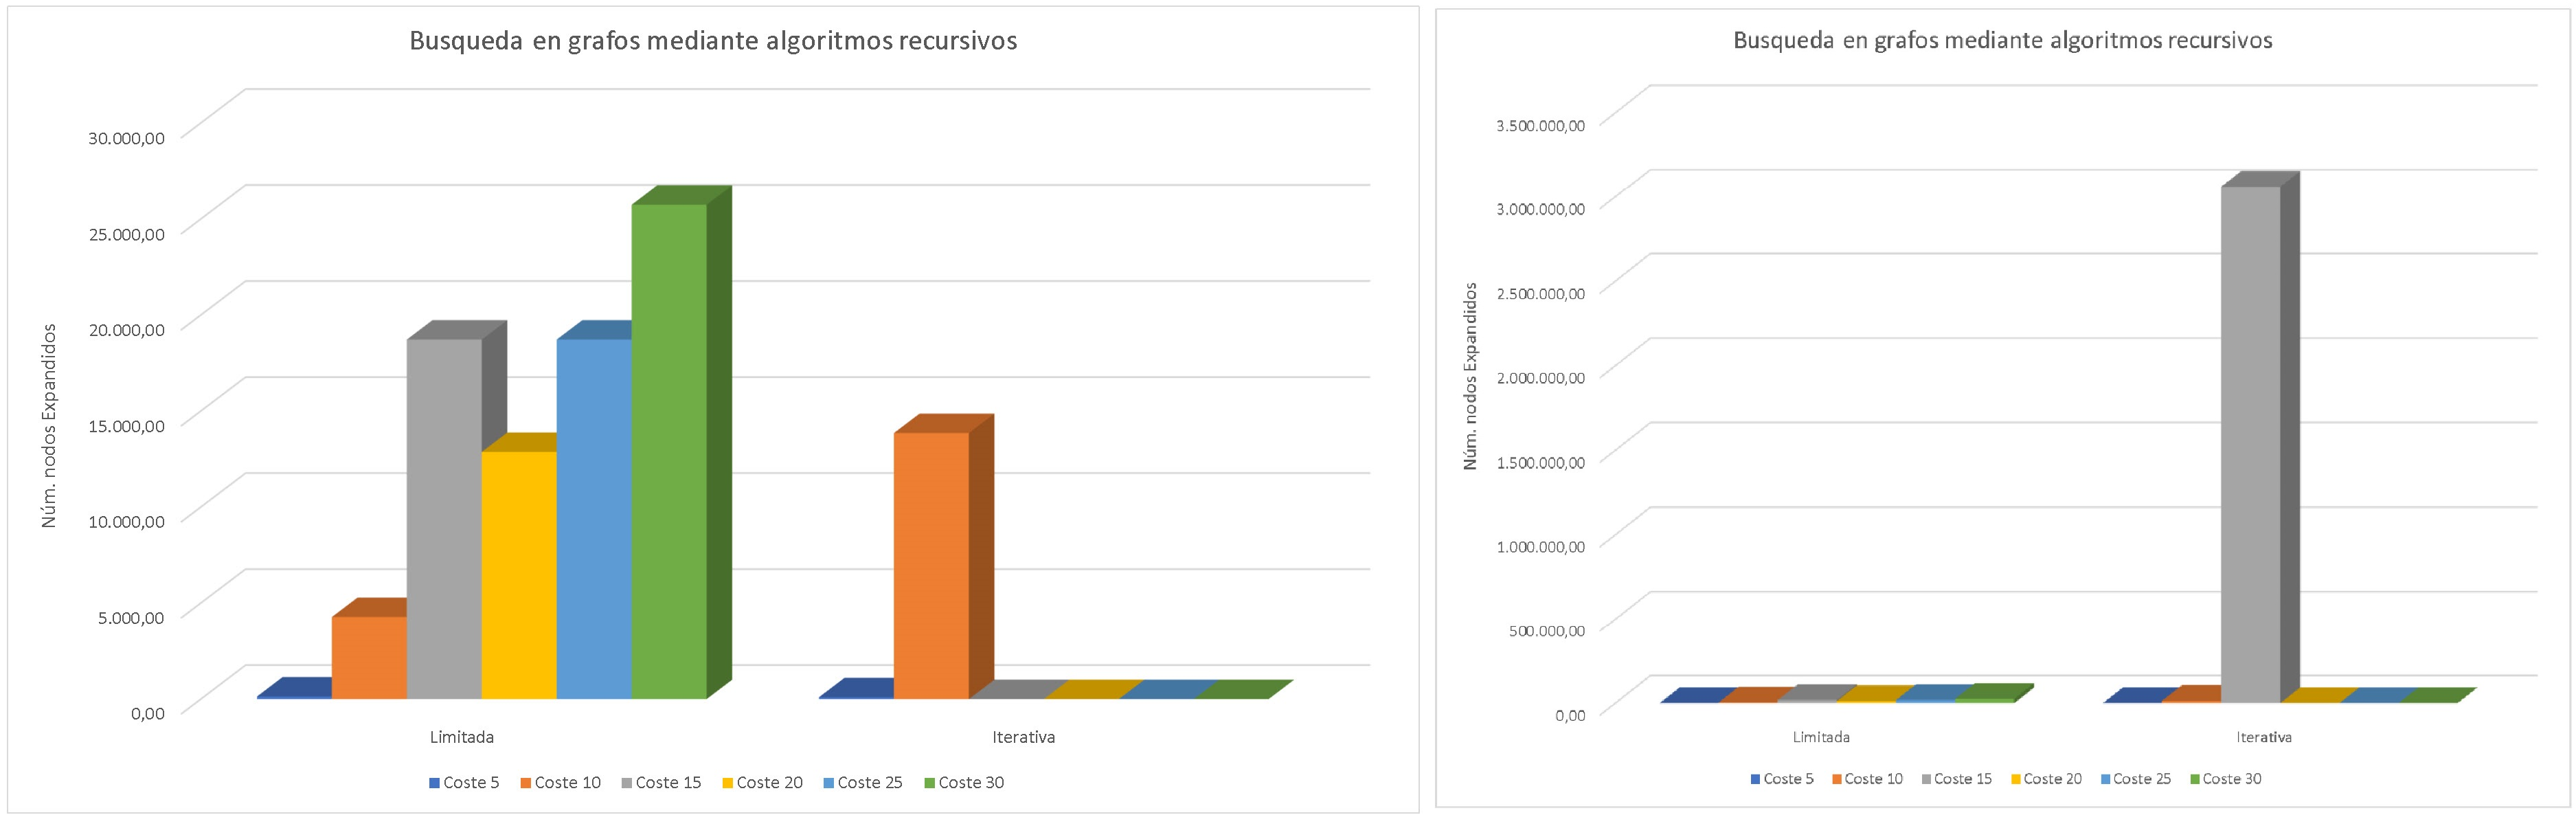
\includegraphics[width=\textwidth]{ejercicio2_3.jpg}
	\caption{Número medio de nodos expandidos por los algoritmos recursivos  en profundidad limitada e iterativa sobre un grafo.} 
	\label{figura_recursiva_grafo}
\end{figure}

Ahora vamos a analizar los resultados de los algoritmos inteligentes. Para empezar vamos a comprobar los heurísticos $ h_0 $, $ h_1 $ y $ h_2 $ y ver como se comportan. 

A la hora de ejecutarlos, no se notan diferencias destacables en cuanto a los tiempos; si es verdad que el algoritmo Manhattan tarda un poco menos que los demás, pero la diferencia es muy pequeña.

La principal característica que hay entre los diferentes heurísticos se ve cuando comparamos el número de nodos que expanden. Si nos fijamos en la \textbf{Figura \ref{figura_heuristicos_basico}} podemos ver como el heurístico $ h_0 $ es bastante similar a los otros dos en los costes más bajos pero, a medida que aumenta el tamaño del problema, se desmarca de los demás como la peor elección. El heurístico $ h_1 $ es algo mejor, pero sigue creciendo mucho en el número de nodos que expande. Por otro lado el $ h_2 $ se mantiene muy por debajo.

\begin{figure}
	\centering
	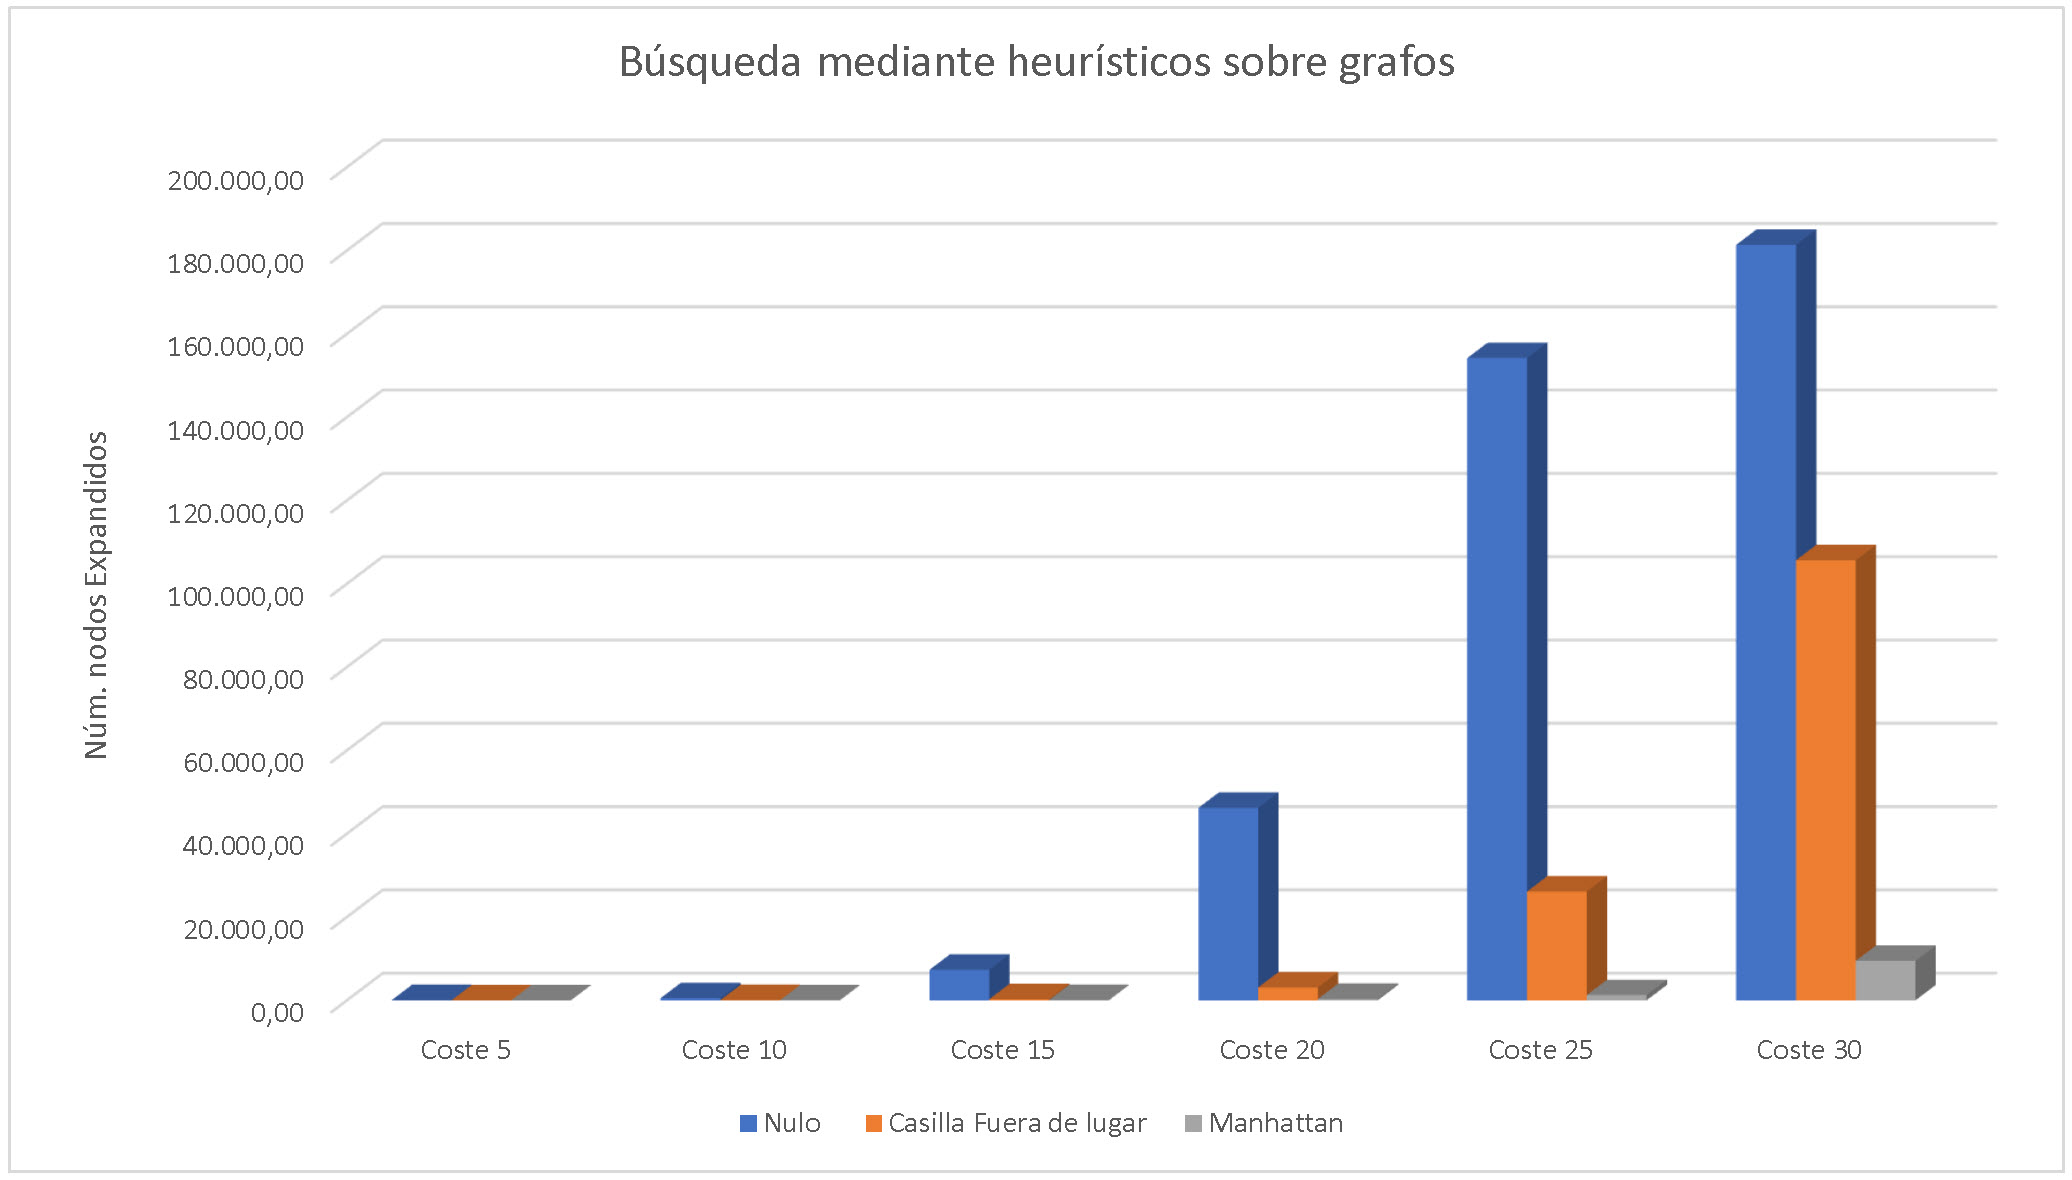
\includegraphics[width=\textwidth]{ejercicio3.jpg}
	\caption{Número medio de nodos expandidos por los algoritmos $ h_0 $, $ h_1 $ y $ h_2 $ sobre un grafo.} 
	\label{figura_heuristicos_basico}
\end{figure}

Cogemos los dos mejores heurísticos del caso anterior y descartamos $ h_0 $ ya que no nos aportara datos relevantes. Ahora comprobaremos la eficacia de $ h_1 $ y $ h_2 $ frente a $ h_{1-2} $, un algoritmo basado en el $ h_1 $, pero con alguna mejora. Al hacer esta nueva comprobación vemos que la \textbf{Figura \ref{figura_heuristicos_1_2}} nos muestra un patrón similar al del caso anterior: $ h_1 $ es peor en tiempo empleado y en número de nodos expandidos, mientras que $ h_{1-2} $, es capaz de reducir ambas métricas dando un mejor resultado; por otro lado $ h_2 $ sigue dominando tanto en tiempo como en número de nodos expandidos.

\begin{figure}
	\centering
	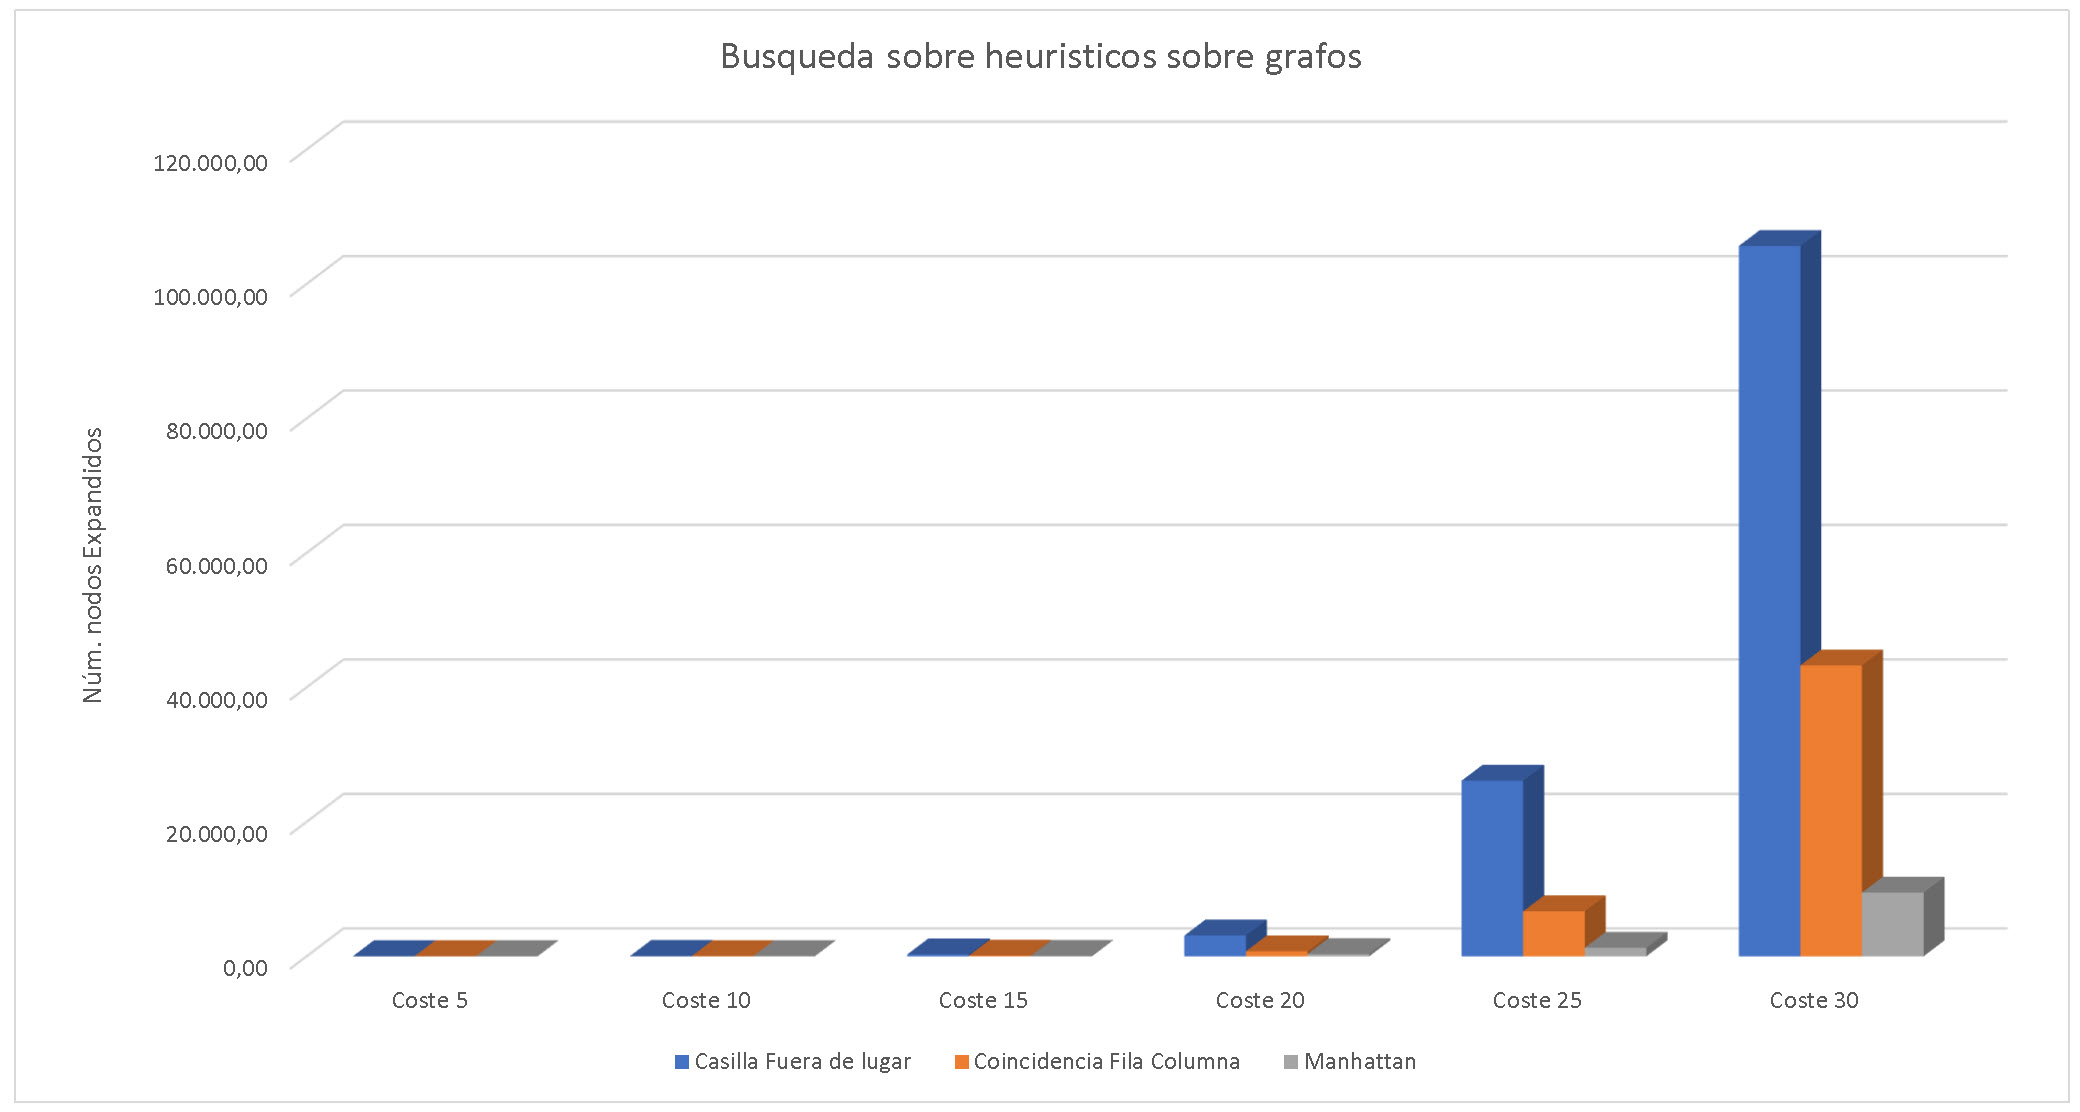
\includegraphics[width=\textwidth]{ejercicio3_2.jpg}
	\caption{Número medio de nodos expandidos por los algoritmos $ h_1 $, $ h_{1-2} $ y $ h_2 $ sobre un grafo.} 
	\label{figura_heuristicos_1_2}
\end{figure}

Ya que el heurístico $ h_2 $ es el mejor hasta ahora, vamos a ver como se comportaría con el caso fallido que tuvimos al principio de nuestras pruebas: búsqueda en espacio de arboles. 

Como muestra la figura \textbf{Figura \ref{figura_Manhattan_arbol}} al principio el número de nodos que expande este heurístico en sus dos versiones es bastante similar, sin embargo, a medida que aumenta el tamaño del problema, el espacio de búsqueda en arboles no nos da resultados viables, a pesar de que estemos utilizando el mejor heurístico.

\begin{figure}
	\centering
	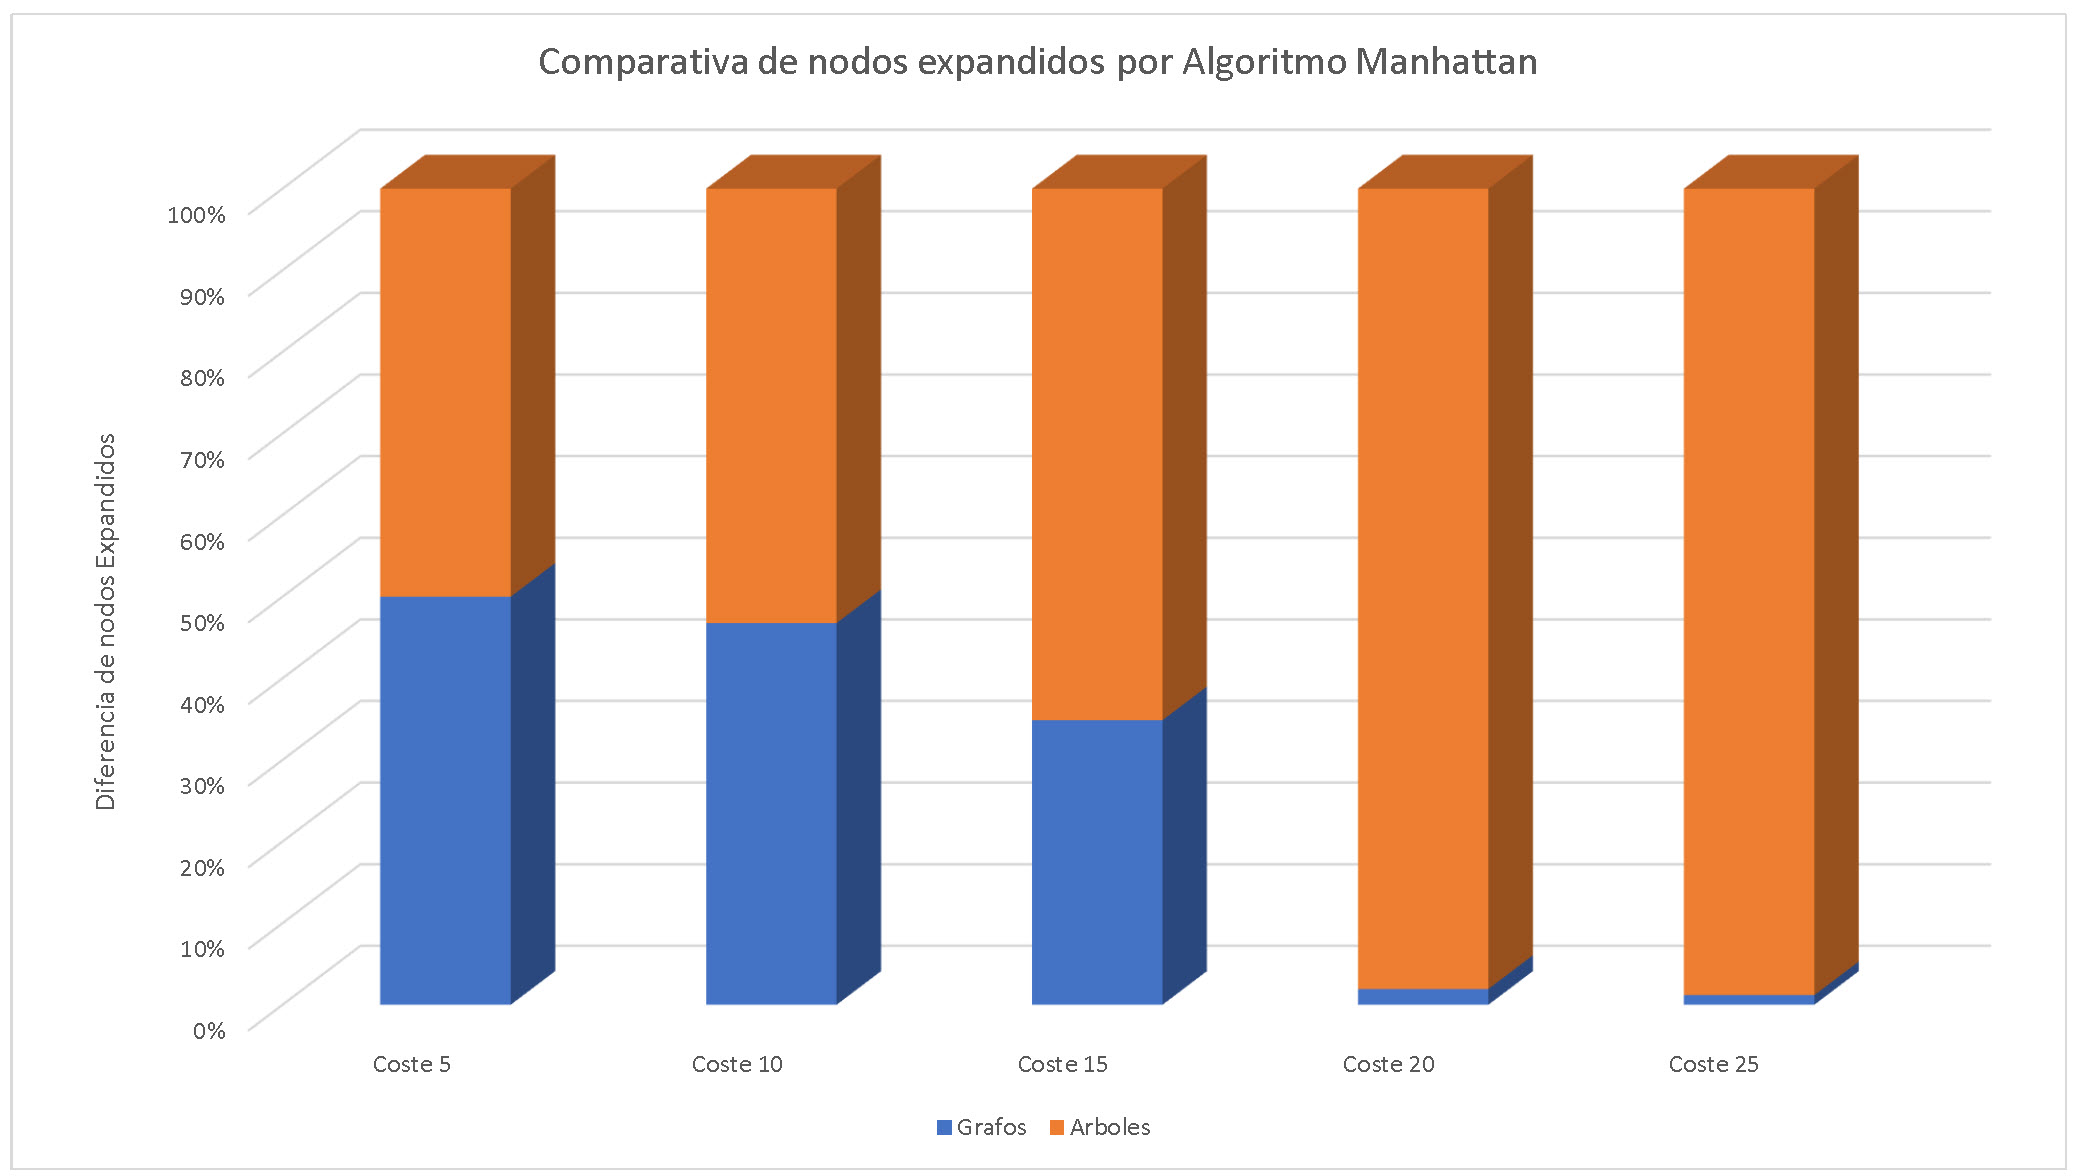
\includegraphics[width=\textwidth]{ejercicio3_3.jpg}
	\caption{Número medio de nodos expandidos por los algoritmos $ h_1 $, $ h_{1-2} $ y $ h_2 $ sobre un grafo.} 
	\label{figura_Manhattan_arbol}
\end{figure}

Hasta ahora hemos probado el algoritmos A* es su versión normal con heurísticos admisibles pero, vamos a probar que resultados nos muestran los algoritmos $ h_2 $ y $ h_3 $ con las versiones con rectificación y re-inserción, lo que puede que nos muestre resultados no óptimos para $ h_3 $.

Para $ h_2 $ no hay mayor cambio al trabajar con estas nuevas versiones de los algoritmos ni tampoco para $ h_3 $. Ambos heurísticos expanden un numero similar de nodos y sus tiempos no sufren grandes variaciones con ninguna de las opciones. En cuanto a cantidad de nodos expandidos, $ h_2 $ sigue siendo mejor en este caso.

Nuestro siguiente paso es ver como se comporta la variante PEA* en función del $\varepsilon$ que se le pase; probaremos con 0.1, 0.5 y 1.0. Como se muestra en la \textbf{Figura \ref{figura_PEA}} a menor cota de error, mayor será el número de nodos expandidos y el tiempo empleado. Aún así, todas las versiones mejoran en la cantidad de nodos expandidos frente a su versión base $ h_2 $.

\begin{figure}
	\centering
	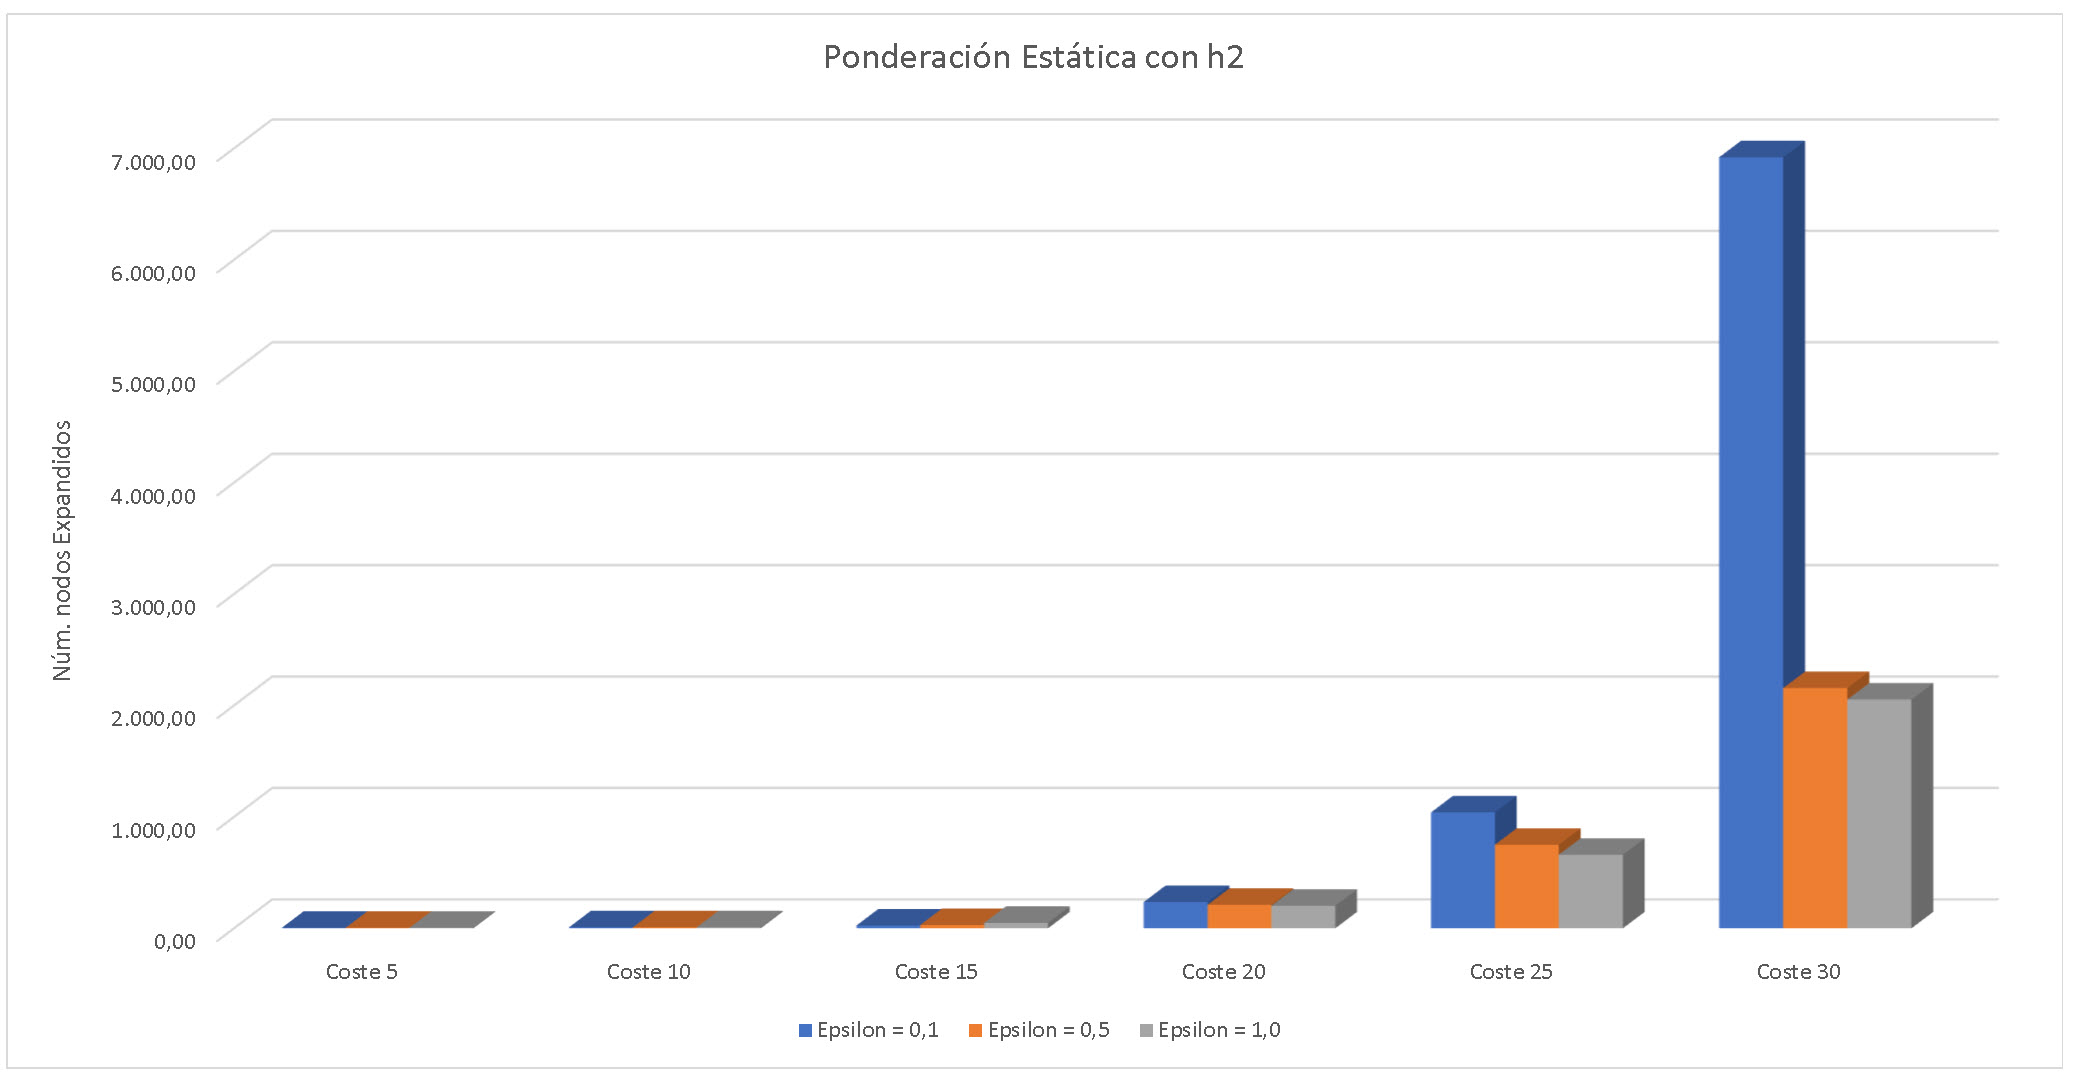
\includegraphics[width=\textwidth]{ejercicio5.jpg}
	\caption{Número medio de nodos expandidos por PEA* sobre un grafo en función de $\varepsilon$.} 
	\label{figura_PEA}
\end{figure}

Para terminar la comparativa entre heurísticos vamos a probar los resultados de nuestro algoritmo $ h_4 $ frente al Greedy Best-First. Como muestra la \textbf{Figura \ref{figura_Greedy}}, GBF es muy superior en cuanto a nodos expandidos; y ésto no repercute en el tiempo que necesita para alcanzar la solución, sin embargo, esta variante no nos proporciona las soluciones optimas mientras que $ h_4 $ si lo hace.

\begin{figure}
	\centering
	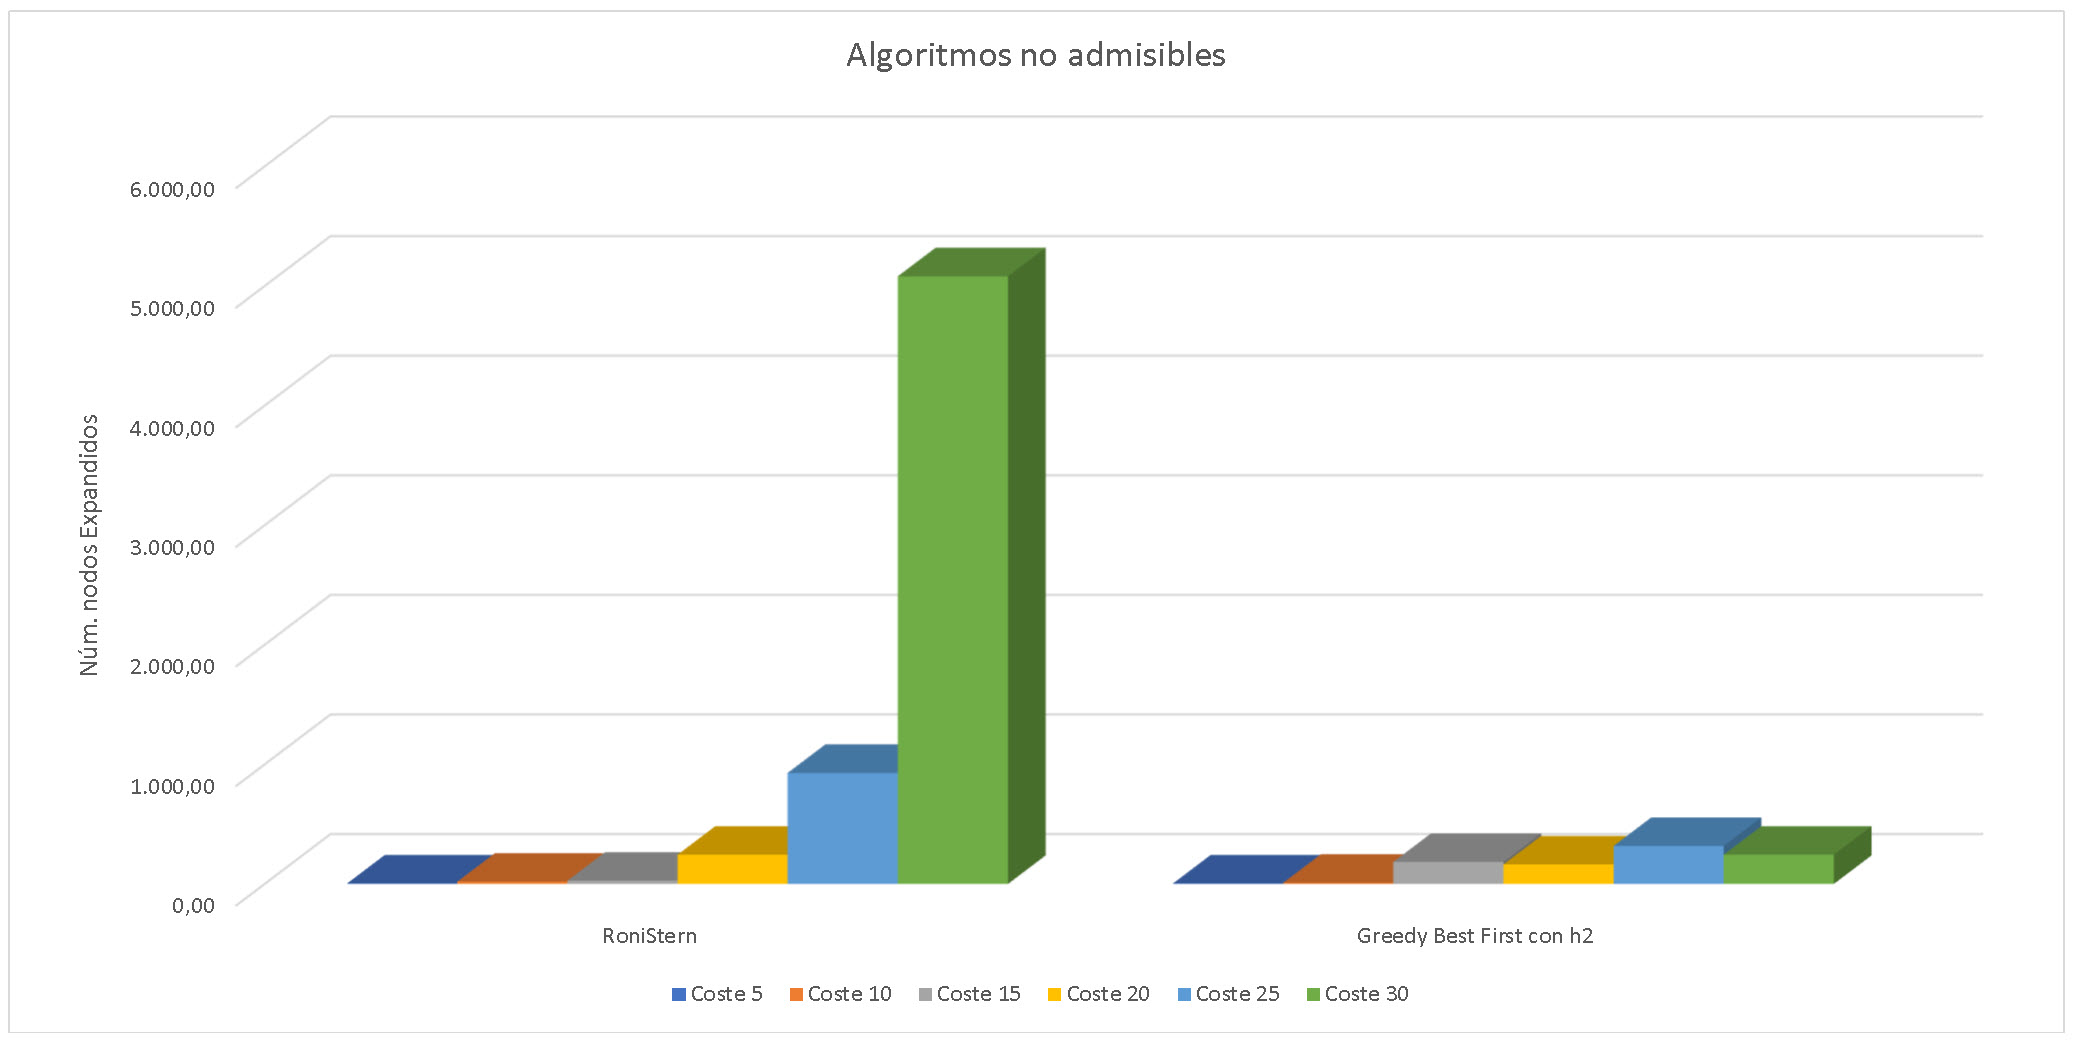
\includegraphics[width=\textwidth]{ejercicio6.jpg}
	\caption{Número medio de nodos expandidos por $ h_4 $ y el Greedy Best-First sobre un grafo.} 
	\label{figura_Greedy}
\end{figure}

Para terminar nuestro experimento vamos a probar un nuevo problema, el problema del viajante de comercio al cual nos referiremos a partir de ahora como TSP y del cual puedes encontrar más información aquí~\cite{referencia_TSP}. Para este nuevo problema vamos a comparar dos nuevos heurísticos: el árbol de expansión mínimo, que puedes descubrir aquí~\cite{referencia_Arbol_Expansion} y el sumatorio minimo de arcos. Enfrentadose a estos dos heuristicos pondremos un algoritmo genético, del cual puedes aprender más aquí~\cite{referencia_Algoritmo_Genetico}. Para el primer caso del algoritmo genético hemos utilizado una probabilidad de mutación de 0.1 y una probabilidad de cruce de 0.8, mientras que para el segundo hemos utilizado una probabilidad de mutación de 0.2 y una probabilidad de cruce de 0.9; para ambos casos se han utilizado 100 generaciones y un tamaño de población de 100 individuos.

Como nos muestra la \textbf{Figura \ref{figura_TSP}}, los resultados de la búsqueda genética no son óptimos pero son bastante buenos, mientras que los heurísticos pueden no llegar a resolverlo en un tiempo razonable.

\begin{figure}
	\centering
	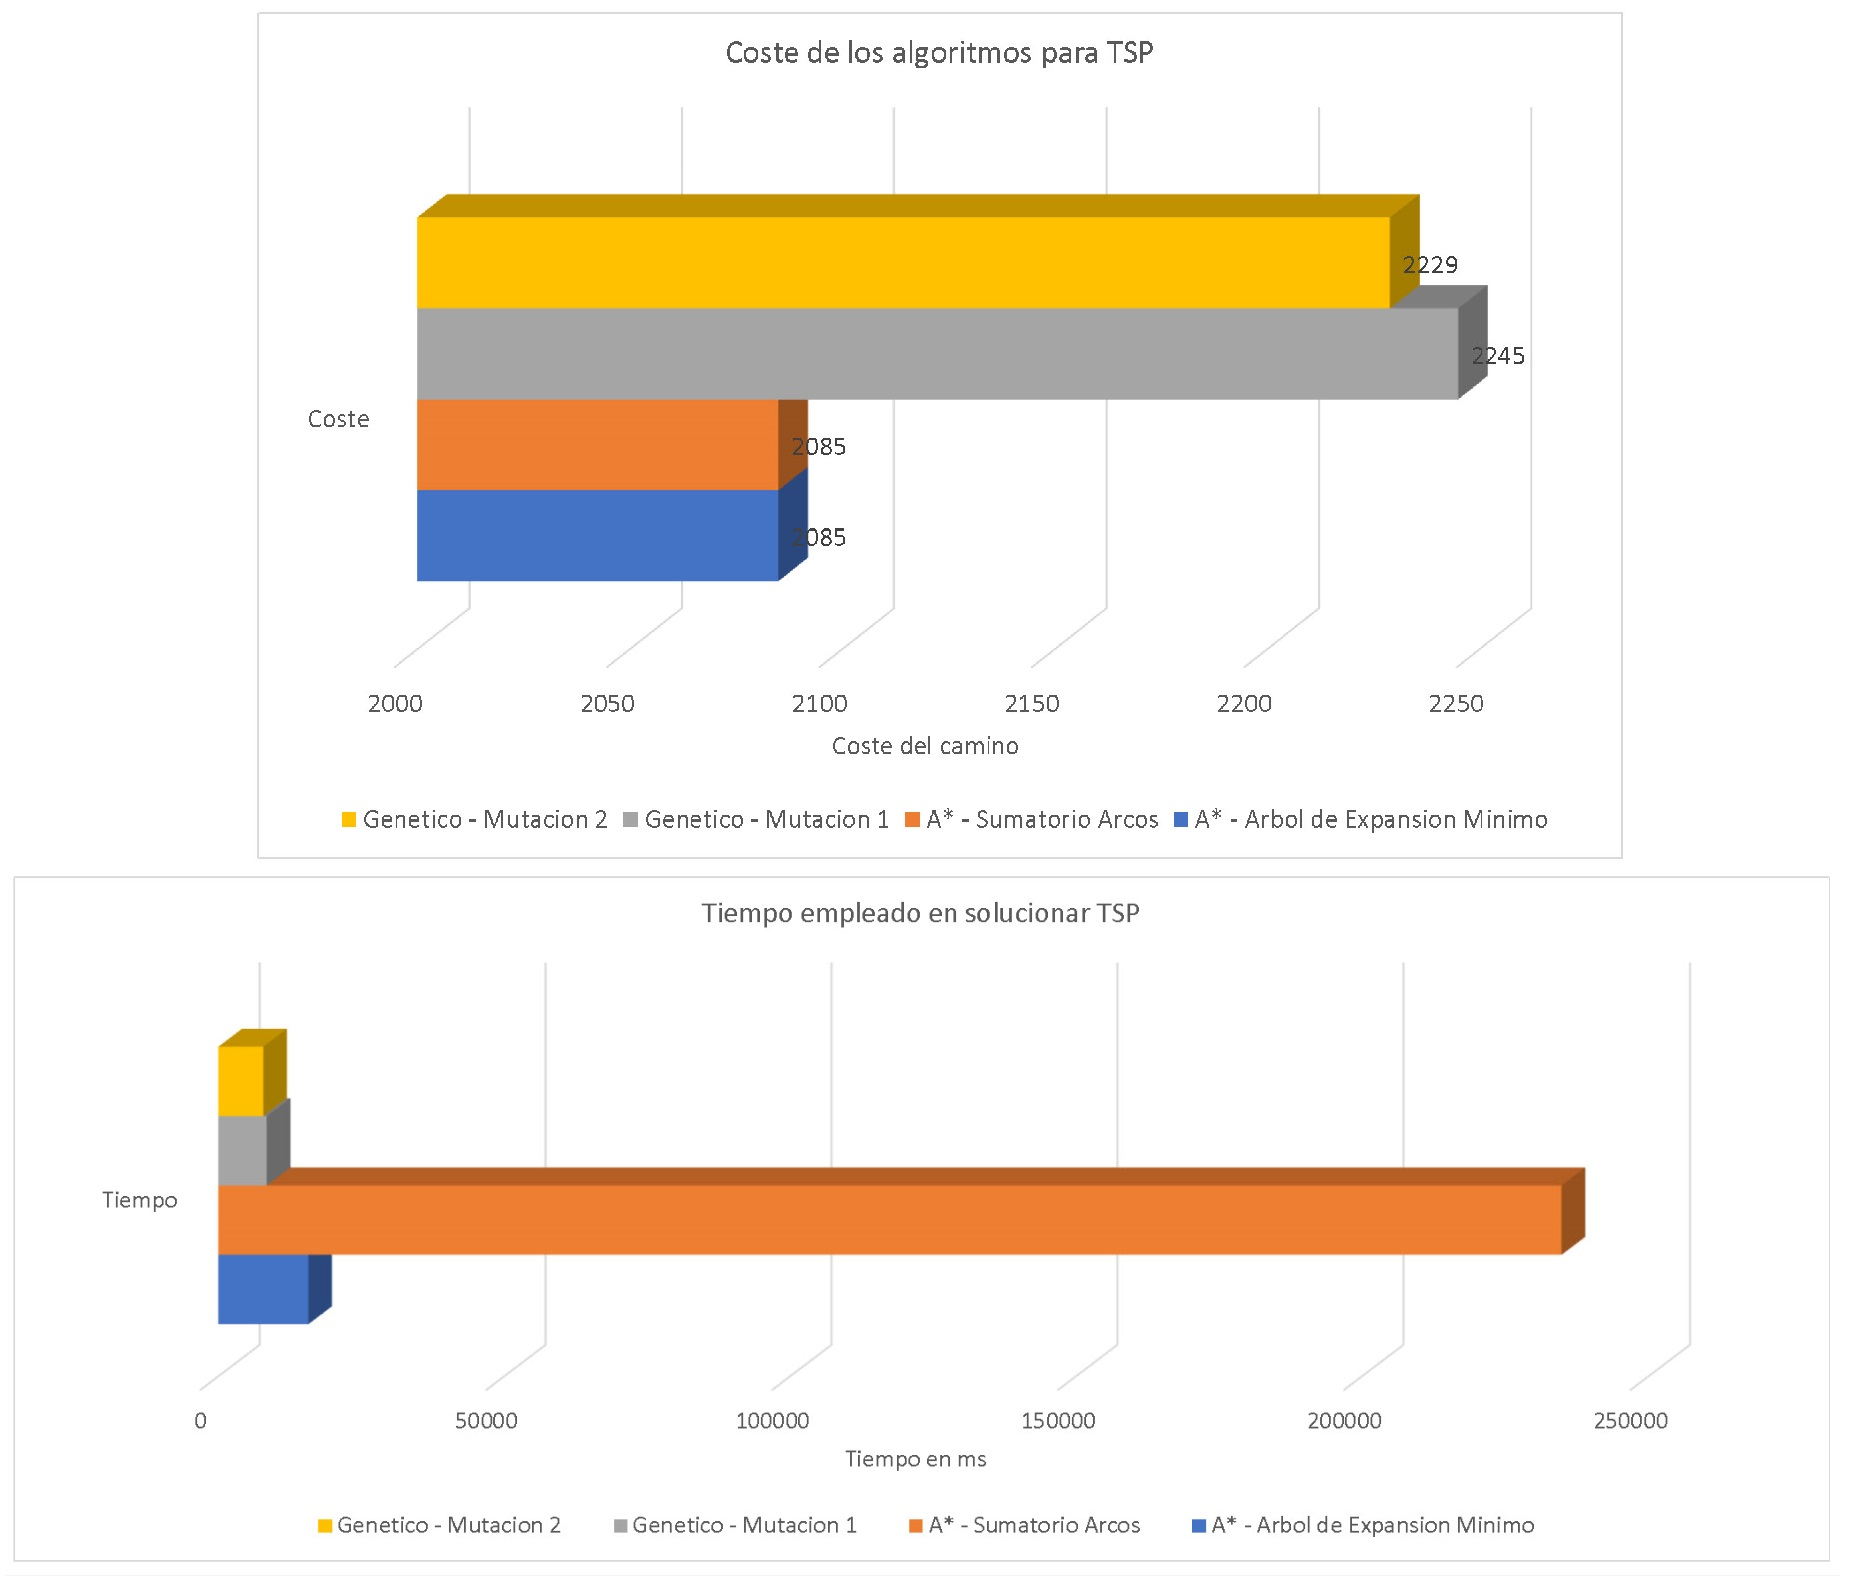
\includegraphics[width=\textwidth]{ejercicio7_3.jpg}
	\caption{Coste medio y tiempo medio que emplearon los algoritmos heurísticos y el genético es sus variantes para resolver el problema del TSP.} 
	\label{figura_TSP}
\end{figure}

\section{Conclusiones}\label{seccion_conclusion}

Por un lado, vemos que los algoritmos de búsqueda a ciegas no tienen cabida en este problema, ya que se ven ampliamente superados por los heurísticos o simplemente no encuentran una solución.
Por otro lado, con el algoritmo A* hemos comprobado que podemos alcanzar soluciones optimas pero que es necesario escoger bien el heurístico adecuado, siendo en nuestro caso $ h_2 $. Para las variaciones de este algoritmo, hemos encontrado que PEA* puede que no nos devuelva una solución optima, pero si valida con la ventaja en el ahorro computacional.
Por ultimo hemos visto que los algoritmos genéticos tampoco nos dan soluciones optimas, pero la diferencia de tiempo frente a los heurísticos, puede suplir la diferencia si así nos conviene. 

\begin{thebibliography}{8}
\bibitem{referencia_Russell}
Stuart Russell, Peter Norvig. Inteligencia Artificial: Un Enfoque Moderno. 2ª
Edición. Prentice Hall, 2004.

\bibitem{referencia_Korf_8}
J.T. Palma y R. Marín (Coordinadores). Inteligencia Artificial: técnicas,
métodos y aplicaciones, McGrawHill, 2008. Capitulo 8.

\bibitem{referencia_Busqueda_Ciegas}
Smart Computing - Gerardo Rossel, \url{http://smartcomputing.gerardorossel.org/busqueda-a-ciegas.aspx}. Ultima modificación 29 Junio 2010

\bibitem{referencia_Korf_9}
J.T. Palma y R. Marín (Coordinadores). Inteligencia Artificial: técnicas,
métodos y aplicaciones, McGrawHill, 2008. Capitulo 9.

\bibitem{referencia_Nilsson}
Nilsson, N., Principles of Artificial Intelligence, Tioga, Palo Alto, CA, 1980.

\bibitem{referencia_Pearl}
Pearl, J., Heuristics, Morgan Kauffman, San Francisco, CA, 1983.

\bibitem{referencia_Geek}
Geeks for Geeks, \url{https://www.geeksforgeeks.org/best-first-search-informed-search}. Ultima modificación 15 Septiembre 2017

\bibitem{referencia_Stern}
R. Stern et al. / Artificial Intelligence 214 (2014) 1-25

\bibitem{referencia_TSP}
Salvador Peñalva García, "El problema del viajante. Métodos de resolución y un enfoque hacia la Teoría de la Computación", \url{https://biblioteca.unirioja.es/tfe\_e/TFE001031.pdf}. Logroño, Julio 2015.

\bibitem{referencia_Arbol_Expansion}
Francisco José Veiga Losada, "El problema del viajante", \url{http://eio.usc.es/pub/mte/descargas/ProyectosFinMaster/Proyecto\_774.pdf}. Santiago de Compostela, 2 Septiembre 2013.

\bibitem{referencia_Algoritmo_Genetico}
\url{https://www.cs.us.es/cursos/ia1-2011/trabajos/propuesta-gen-tsp.html}.

\end{thebibliography}

\end{document}